\documentclass[twoside,a4paper]{article}
% \usepackage{enumerate}
% \setbeamertemplate{enumerate item}{(\alph{enumi})}
% \setbeamertemplate{enumerate subitem}{(\roman{enumii})}


%% Packages
\usepackage{xfrac}
\usepackage{amsmath}
\usepackage{amsfonts}
\usepackage{amssymb}
\usepackage{amsbsy}
\usepackage{amsthm}
\usepackage{isomath}
\usepackage{algorithm}
\usepackage{algorithmic}
\usepackage{mathrsfs}
\usepackage{dsfont}
\usepackage{epic}
\usepackage{pstool}

%%%% FOR WIDE TILDE %%%%
\usepackage{scalerel}
\usepackage{stackengine,wasysym}

\newcommand\reallywidetilde[1]{\ThisStyle{%
\setbox0=\hbox{$\SavedStyle#1$}%
\stackengine{-.1\LMpt}{$\SavedStyle#1$}{%
\stretchto{\scaleto{\SavedStyle\mkern.2mu\AC}{.5150\wd0}}{.6\ht0}%
}{O}{c}{F}{T}{S}%
}}


%\usepackage[bbgreekl]{mathbbol}
\usepackage{subfigure}
\usepackage{tikz}

%\usetikzlibrary{external}
%\tikzexternalize[prefix=tikz/]
\usepackage{gnuplot-lua-tikz}
\usepackage{pgfplots}
\usepackage{colortbl}
\usepackage{enumerate}
\usepackage[pdfauthor={Christos Dimitrakakis and Ronald Ortner},
pdftitle={Decision Making Under Uncertainty and Reinforcement Learning},
pdfsubject={Decision theory},
pdfkeywords={Reinforcement Learning, Decision Theory, Machine Learning, Statistics, Game Theory},
pdfproducer={Latex with hyperref},
pdfcreator={LaTex},
pdfpagelabels]{hyperref}


\usepackage{cleveref}


%\usepackage[sort&compress]{natbib}
\usepackage{natbib}

%\usepackage{epstopdf}

\newcommand \indexmargin[1] {\marginpar{\emph{#1}}\index{#1}}
\newcommand \marginref[2] {\marginpar{\emph{#1}}\emph{#1}\index{#2}}
\newcommand \emindex[1] {\emph{#1}\marginpar{\emph{#1}}\index{#1}}
\newcommand \justindex[1] {\emph{#1}\index{#1}}

%% Special characters

\DeclareSymbolFont{bbold}{U}{bbold}{m}{n}
\DeclareSymbolFontAlphabet{\mathbbold}{bbold}

\newcommand\Reals {{\mathds{R}}}
\newcommand\Simplex {\mathbbold{\Delta}}
\newcommand\PSD {{\mathds{S}}}
\newcommand\Naturals {{\mathds{N}}} 
\newcommand\Integers {{\mathds{Z}}} 

\newcommand \FB {{\mathfrak{B}}}
\newcommand \FD {{\mathfrak{D}}}
\newcommand \FF {{\mathfrak{F}}}
\newcommand \FK {{\mathfrak{K}}}
\newcommand \FJ {{\mathfrak{J}}}
\newcommand \FL {{\mathfrak{L}}}
\newcommand \FO {{\mathfrak{O}}}
\newcommand \FS {{\mathfrak{S}}}
\newcommand \FT {{\mathfrak{T}}}
\newcommand \FP {{\mathfrak{P}}}
\newcommand \FR {{\mathfrak{R}}}

\newcommand \Borel[1] {\mathfrak{B}\left(#1\right)}
\newcommand \Dist[1] {\Simplex \left(#1\right)}

\newcommand \CA {{\mathcal{A}}}
\newcommand \CB {{\mathcal{B}}}
\newcommand \CC {{\mathcal{C}}}
\newcommand \CD {{\mathcal{D}}}
\newcommand \CE {{\mathcal{E}}}
\newcommand \CF {{\mathcal{F}}}
\newcommand \CG {{\mathcal{G}}}
\newcommand \CH {{\mathcal{H}}}
\newcommand \CJ {{\mathcal{J}}}
\newcommand \CL {{\mathcal{L}}}
\newcommand \CM {{\mathcal{M}}}
\newcommand \CN {{\mathcal{N}}}
\newcommand \CO {{\mathcal{O}}}
\newcommand \CP {{\mathcal{P}}}
\newcommand \CQ {{\mathcal{Q}}}
\newcommand \CR {{\mathcal{R}}}
\newcommand \CS {{\mathcal{S}}}
\newcommand \CT {{\mathcal{T}}}
\newcommand \CU {{\mathcal{U}}}
\newcommand \CV {{\mathcal{V}}}
\newcommand \CW {{\mathcal{W}}}
\newcommand \CX {{\mathcal{X}}}
\newcommand \CY {{\mathcal{Y}}}
\newcommand \CZ {{\mathcal{Z}}}

\newcommand \BA {{\mathbb{A}}}
\newcommand \BI {{\mathbb{I}}}
\newcommand \BS {{\mathbb{S}}}

\newcommand \bR {{\vectorsym{R}}}
\newcommand \bS {{\vectorsym{S}}}
\newcommand \bT {{\vectorsym{T}}}
\newcommand \bU {{\vectorsym{U}}}
\newcommand \bV {{\vectorsym{V}}}

\newcommand \bz {{\vectorsym{z}}}
\newcommand \bx {{\vectorsym{x}}}
\newcommand \by {{\vectorsym{y}}}
\newcommand \bu {{\vectorsym{u}}}
\newcommand \bw {{\vectorsym{w}}}
\newcommand \ba {{\vectorsym{a}}}
\newcommand \bh {{\vectorsym{h}}}
\newcommand \bo {{\vectorsym{o}}}
\newcommand \bn {{\vectorsym{n}}}
\newcommand \bp {{\vectorsym{p}}}
\newcommand \bq {{\vectorsym{q}}}
\newcommand \bs {{\vectorsym{s}}}

\newcommand \SA {\mathscr{A}}
\newcommand \SB {\mathscr{B}}
\newcommand \SC {\mathscr{C}}
\newcommand \SF {\mathscr{F}}
\newcommand \SG {\mathscr{G}}
\newcommand \SH {\mathscr{H}}
\newcommand \SJ {\mathscr{J}}
\newcommand \SL {\mathscr{L}}
\newcommand \SP {\mathscr{P}}
\newcommand \SR {\mathscr{R}}
\newcommand \ST {\mathscr{T}}
\newcommand \SU {\mathscr{U}}
\newcommand \SV {\mathscr{V}}
\newcommand \SW {\mathscr{W}}

\newcommand \p {\partial}
\newcommand \deriv[1] {\nabla_{#1}}




\newcommand\then{\Rightarrow}
%\newcommand \StateSet {{\CQ}}
\newcommand \States {\CS}
\newcommand \Actions {\CA}

\newcommand \stat {\phi}

%% Commands

\newcommand\argmax{\mathop{\rm arg\,max}}
\newcommand\argmin{\mathop{\rm arg\,min}}
\newcommand\dtan{\mathop{\rm dtan}}
\newcommand\sgn{\mathop{\rm sgn}}
\newcommand\trace{\mathop{\rm trace}}
\newcommand\diag{\mathop{\rm diag}}
%\newcommand\dim{\mathop{\rm dim}}
\newcommand\sinc{\mathop{\rm sinc}}


\newcommand\ind[1]{\mathop{\mbox{\ensuremath{\mathbb{I}}}}\left\{#1\right\}}
\newcommand\Ind{\mbox{\bf{I}}}
\newcommand\I[1]{\mathop{\mbox{\ensuremath{\mathbbold{1}_{#1}}}}}

\newcommand \E {\mathop{\mbox{\ensuremath{\mathbb{E}}}}\nolimits}
\newcommand \hE {\mathop{\mbox{\ensuremath{\hat{\mathbb{E}}}}}\nolimits}
\newcommand \Var {\mathop{\mbox{\ensuremath{\mathbb{V}}}}\nolimits}
\renewcommand \Pr {\mathop{\mbox{\ensuremath{\mathbb{P}}}}\nolimits}
%\newcommand \complement[1] {\bar{#1}}
\newcommand \transpose[1] {#1^\top}
\newcommand \pinv[1] {\reallywidetilde{#1}^{-1}}
\newcommand \inv[1] {#1^{-1}}
\newcommand \defn {\mathrel{\triangleq}}
\newcommand\set[1] {\left\{#1\right\}}
\newcommand\tuple[1] {\left\langle #1\right\rangle}
\newcommand\cset[2] {\left\{#1 ~\middle|~ #2\right\}}
\newcommand \ceil[1]{\left\lceil #1 \right\rceil}
\newcommand \floor[1]{\left\lfloor #1 \right\rfloor}
\newcommand \norm[1]{\left\|#1\right\|}
\newcommand \pnorm[2]{\left\|#1\right\|_{#2}}
\newcommand \meas[1]{\mu\left\{#1\right\}}
\newcommand \dd{\, \mathrm{d}}
\newcommand \eq {=}

\newcommand \setdiff {\mathrel{\triangle}}

\newcommand \KL[2] {D\left( #1 ~\middle\|~ #2 \right)}

\numberwithin{equation}{section}


\theoremstyle{plain}
\newtheorem{assumption}{Assumption}
\newtheorem{lemma}{Lemma}
\newtheorem{theorem}{Theorem}
\newtheorem{corollary}{Corollary}
\theoremstyle{definition}
\newtheorem{definition}{Definition}
\theoremstyle{remark}
\newtheorem{remark}{Remark}
%%% Examples %%%%
\newtheoremstyle{example}  % Name
{1em}       % Space above 
{1em}       % Space below
{\small}      % Body font
{}          % Indent amount 
{\scshape}  % Theorem head font
{.}         % Punctuation after theorem head
{.5em}      % Space after theorem head
{}          % Theorem head spec
\theoremstyle{example}
\newtheorem{example}{Example}
\newtheorem{exercise}{Exercise}


\newcommand \eqlike {\eqsim}
\newcommand \gtlike {\succ}
\newcommand \ltlike {\prec}
\newcommand \gelike {\succsim}
\newcommand \lelike {\precsim}

\newcommand \eqpref {\eqsim^*}
\newcommand \gtpref {\succ^*}
\newcommand \ltpref {\prec^*}
\newcommand \gepref {\succsim^*}
\newcommand \lepref {\precsim^*}

\newcommand \Util {U}
\newcommand \BUtil {U^*}
\newcommand \MUtil {\matrixsym{U}}
\newcommand \risk {\kappa}
\newcommand \Brisk {\kappa^*}
\newcommand \Loss {\ell}
\newcommand \Regret {L}
\newcommand \regret {\ell}
\newcommand \act {a}
\newcommand \Acts {\CA}
%% Make decisions and decision functions synonyms to actions and policies
\newcommand \decision {\act}
\newcommand \Decisions {\Acts}
\newcommand \stopfun {\decfun_s}
\newcommand \decrule {\decfun_d}
\newcommand \strategy {\sigma}
\newcommand \Strategies {\Sigma}
\newcommand \decfun {\pol}
\newcommand \Decfuns {\Pols}
%\newcommand \dprior {\pi}
%\newcommand \DPriors {\Pi}

\DeclareMathAlphabet{\mathpzc}{OT1}{pzc}{m}{it}

\newcommand \Softmax {{\mathpzc{Softmax}}}
\newcommand \GammaDist {{\mathpzc{Gamma}}}
\newcommand \Dirichlet {{\mathpzc{Dir}}}
\newcommand \Uniform {{\mathpzc{Unif}}}
\newcommand \Bernoulli {{\mathpzc{Bern}}}
\newcommand \Binomial {{\mathpzc{Binom}}}
\newcommand \Beta {{\mathpzc{Beta}}}
\newcommand \Geometric {{\mathpzc{Geom}}}
\newcommand \Normal {{\mathpzc{N}}}
\newcommand \Multinomial {{\mathpzc{Mult}}}
\newcommand \Wishart {{\mathpzc{Wish}}}



\newcommand \rmax {r_\mathrm{max}}

\newcommand \ident {\matrixsym{I}}
\newcommand \trans {\matrixsym{P}}
\newcommand \rew {\vectorsym{r}}
\newcommand \RewValues {\mathcal{R}}
\newcommand \Rew {\rho}
\newcommand \Rews {\mathscr{R}}

\newcommand \agrew {\rew_{\mathrm{a}}}
\newcommand \agpol {\pol_{\mathrm{a}}}

\newcommand \temp {\eta}
\newcommand \gammaA {\zeta}
\newcommand \gammaB {\theta}

\newcommand \outcome {\omega}
\newcommand \Outcomes {\Omega}

\newcommand \vomega {\vectorsym{\omega}}

\newcommand \hbel {\omega}
\newcommand \jbel {\phi}
\newcommand \rbel {\xi}
\newcommand \pbel {\psi}


\newcommand \aval {\vectorsym{u}}
\newcommand \Value {V}
\newcommand \val {\vectorsym{v}}
\newcommand \Vals {\mathcal{V}}
\newcommand \qval {\vectorsym{q}}
\newcommand \Qvals {\mathcal{Q}}
\newcommand \blm {\mathscr{L}}
\newcommand \tdm {\mathscr{D}}
\newcommand \pim {\mathscr{B}}
\newcommand \disc {\gamma}
\newcommand \hist {h_t}

\newcommand \horizon {T}

\newcommand \Pmp {\Pr_\mdp^\pol}
\newcommand \pol {\pi}
\newcommand \Pols {\Pi}
\newcommand \vpol {\vectorsym{\pol}}
\newcommand \marginal {P_\bel}
\newcommand \nmarginal[1] {P_{\bel_{#1}}}
\newcommand \bel {\xi}
\newcommand \Bels {\Xi}
\newcommand \field {\CF}
\newcommand \family {\SP}
\newcommand \funfamily {\SF}
\newcommand \vbel {\vectorsym{\bel}}
\newcommand \mdp {\mu}
\newcommand \MDPs {\CM}
\newcommand \hmdpt {\widehat{\mdp_t}}
\newcommand \hmdp {\widehat{\mdp}}
\newcommand \meanMDP[1][\bel] {\hmdp(#1)}
\newcommand \maxMDP[1][\bel] {\hmdp^*(#1)}
\newcommand \cmp {\nu}
\newcommand \CMPs {\CN}
\newcommand \POMDPs {\CM_{P}}
\newcommand \hyper {\psi}
\newcommand \Hypers {\Psi}

\newcommand \opol {\beta}
\newcommand \ot {\beta_t}

\newcommand \Ct {M_t}
\newcommand \Trans {\CT}
\newcommand \tran[2] {\trans(#1 \mid #2)}
\newcommand \Tpl {\Trans_\pol}
\newcommand \hTpl {\hat{\Trans}_\pol}
\newcommand \htran[2] {\hat{\trans}_t(#1 \mid #2)}
\newcommand \visits[1] {N_t(#1)}
\newcommand \Statedist {\matrixsym{X}}
\newcommand \statedist {x}
\newcommand \statedists {\vectorsym{x}}
\newcommand \start {y} % starting state distribution
\newcommand \starts {\vectorsym{y}} % starting state distribution

\newcommand \noise {\vectorsym{\varepsilon}}
\newcommand \MW {\matrixsym{W}}
\newcommand {\MH} {\matrixsym{H}}
\newcommand {\MK} {\matrixsym{K}}
\newcommand {\MR} {\matrixsym{R}}

\newcommand \MB {\matrixsym{B}}
\newcommand \MV {\matrixsym{V}}
\newcommand \vs {\vectorsym{s}}
\newcommand \vx {\vectorsym{x}}
\newcommand \vm {\vectorsym{m}}


\newcommand \basis {f}
\newcommand \mbel {\phi}

\newcommand \pmean {\matrixsym{M}}
\newcommand \pcov {\matrixsym{C}}
\newcommand \pwish {\matrixsym{W}}

\newcommand \MA {\matrixsym{A}}
\newcommand \feat {\matrixsym{\Phi}}
\newcommand \vb {\vectorsym{b}}
\newcommand \vp {\vectorsym{p}}
\newcommand \MP {\matrixsym{P}}
\newcommand \vparam {\vectorsym{\theta}}
\newcommand \MParam {\matrixsym{\Theta}}
\newcommand \param {\theta}
\newcommand \Params {\Theta}
\newcommand \vpparam {\vectorsym{\alpha}}
\newcommand \pparam {\alpha}
\newcommand \PParams {A}

\newcommand \elig {\vectorsym{e}}
\newcommand \step {\alpha}

\newcommand \eit {f_{i,t}}
\newcommand \pt {\pol_t}
\newcommand \rt {r_t}
\newcommand \rit {r_{i,t}}
\newcommand \st {s_t}
\newcommand \sT {s^T}
\newcommand \xt {x_t}
\newcommand \xT {x^T}
\newcommand \at {a_t}
\newcommand \aT {a^T}
\newcommand \yt {y_t}
\newcommand \yT {y^T}

\newcommand \nactions {k}
\newcommand \nstates{n}
\newcommand \nobservations {m}

\newcommand \figwidth {0.6\textwidth}
\newcommand \figheight {0.4\textwidth}

%%% macros to make things smalller
% For comparison, the existing overlap macros:
% \def\llap#1{\hbox to 0pt{\hss#1}}
% \def\rlap#1{\hbox to 0pt{#1\hss}}
\def\clap#1{\hbox to 0pt{\hss#1\hss}}
\def\mathllap{\mathpalette\mathllapinternal}
\def\mathrlap{\mathpalette\mathrlapinternal}
\def\mathclap{\mathpalette\mathclapinternal}
\def\mathllapinternal#1#2{%
\llap{$\mathsurround=0pt#1{#2}$}}
\def\mathrlapinternal#1#2{%
\rlap{$\mathsurround=0pt#1{#2}$}}
\def\mathclapinternal#1#2{%
\clap{$\mathsurround=0pt#1{#2}$}}




\usetikzlibrary{automata}
\usetikzlibrary{topaths}
\usetikzlibrary{shapes}
\usetikzlibrary{arrows}
\usetikzlibrary{decorations.markings}
\usetikzlibrary{intersections}

\tikzstyle{place}=[circle,draw=black,inner sep=0mm, minimum size=6mm]

\tikzstyle{utility}=[diamond,draw=black,draw=blue!50,fill=blue!10,inner sep=0mm, minimum size=8mm]
\tikzstyle{select}=[rectangle,draw=black,draw=blue!50,fill=blue!10,inner sep=0mm, minimum size=6mm]
\tikzstyle{hidden}=[dashed,draw=black,fill=red!10]
\tikzstyle{RV}=[circle,draw=black,draw=blue!50,fill=blue!10,inner sep=0mm, minimum size=6mm]

\tikzstyle{transition}=[rectangle,draw=black!50,fill=black!20,thick]
\tikzstyle{someset}=[circle,draw=black,minimum size=8mm]
\tikzstyle{point}=[circle,draw=black,fill=black]

\def \solution {1}



\pagestyle{myheadings}



\begin{document}
\title{Exercise set 2}

\author{Christos Dimitrakakis: \texttt{christos.dimitrakakis@unine.ch}}

\maketitle
\large{Deadline: 5 March 2024}


\vspace{1em}


\begin{exercise}
  Complete the meteorologists exercise for the Bayesian and Maximum-A-Posteriori models.
\end{exercise}

\begin{exercise}
  Consider a  Bernoulli random variable with unknown mean
  \[
    x_t \mid \mu \sim \Bernoulli(\mu),
  \]
  where the mean is sampled from a Beta distribution
  \[
    \mu \sim \Beta(\alpha, \beta).
  \]
  The Bernoulli distribution satisfies
  \[
    P_\mu(x_1, \ldots, x_T) = \prod_{t=1}^T P_\mu(x_t) = \prod_{t=1}^T \mu^{s_T} (1 - \mu)^{T - s_T},
  \]
  where $s_T = \sum_{t=1}^T x_T$, while the Beta distribution has the form
  \[
    \bel(\mu) \defn \frac{1}{B(\alpha, \beta)} \mu^{\alpha - 1} (1 - \mu)^{\beta - 1},
  \]
  where the factor $B(\alpha, \beta)$ is a normalisation constant independent of $\mu$ that ensures the density integrates to one.
  \begin{enumerate}
  \item Show that the maximum likelihood estimate
    \[
      \argmax_\mu P_\mu(x_1, \ldots, x_T) 
    \]
    is $\mu = s_T/T$.
  \item Show that the maximum a posteriori estimate
    \[
      \argmax_\mu P_\mu(x_1, \ldots, x_T) \bel(\mu)
    \]
    is $\mu = (\alpha + s_T - 1) / (\alpha + \beta + T - 2)$.
  \item Show that the posterior expected value
    \[
      \E_\bel(\mu | x_1, \ldots, x_t) = \int_{-\infty}^\infty \mu \, d \bel(\mu \mid x_1, \ldots, x_T)
    \]
    is $\mu = (\alpha + s_T) / (\alpha + \beta + T)$.
  \end{enumerate}
  
\end{exercise}
\if\solution 1
  \begin{proof}[Exercise 2 solution]
    To make this simpler, we can take the logarithm of the likelihood
    \begin{align*}
      \ln P_\mu(x_1, \ldots, x_T)
      &=  s_T \ln \mu + (T - s_T) \ln (1 - \mu)
    \end{align*}
    Since $\ln$ is a monotonic function, finding the maximum of the log-likelihood is equivalent to finding the maximum of the likelihood. We can do so by taking the derivative and setting it to zero:
    \begin{align*}
      0 &= \frac{d}{d\mu} \ln P_\mu(x_1, \ldots, x_T)\\
        &=  \frac{d}{d\mu} s_T \ln \mu + \frac{d}{d\mu}  (T - s_T) \ln (1 - \mu)\\
        &=   s_T/\mu  - (T - s_T) / (1 - \mu)\\
      \mu &=   s_T /T.
    \end{align*}
    For the \emph{maximum a posteriori} estimate, we can use the same approach
    \begin{align*}
      0 &=\frac{d}{d\mu} \ln [P_\mu(x_1, \ldots, x_T) \bel(\mu)]\\
      &=
        \frac{d}{d\mu} \ln P_\mu(x_1, \ldots, x_T) + \frac{d}{d\mu} \ln \bel(\mu)\\
      &=
        \frac{s_T}{\mu} - \frac{T - s_T}{1 - \mu}
        +
        \frac{\alpha - 1}{\mu} -  \frac{\beta - 1}{1 - \mu}\\
      &=
        \frac{s_T + \alpha - 1}{\mu}  - \frac{T - s_T + \beta - 1}{1 - \mu}\\
      (s_T + \alpha - 1)(1 - \mu) &= (T - s_T + \beta - 1) \mu\\
      (s_T + \alpha - 1)  &= (T + \beta + \alpha - 2 ) \mu\\
      \mu & = \frac{s_T + \alpha - 1}{T + \beta + \alpha - 2 }
    \end{align*}
    Finally, we can look at the expected value of the distribution. Here we can use a shortcut. We know that the expected value of a Beta distribution with parameters $\alpha, \beta$ is $\alpha / (\alpha + \beta)$. Since we now have a Beta distribution with parameters $\alpha + s_T, \beta + T - s_T$, the expected value is $\alpha + s_T / (\alpha + \beta + T)$. We can prove that this is the
    correct expectation as follows:
    \begin{align*}
      1/B(\alpha, \beta)
      \int_0^1 
      \mu \mu^{\alpha- 1}
      (1 - \mu)^{\beta - 1} d\mu
      &=
        B(\alpha + 1, \beta)/B(\alpha, \beta)
    \end{align*}
    The Beta function has the property that $B(\alpha + 1, \beta) = B(\alpha, \beta) \frac{\alpha}{\alpha + \beta}$. Replacing, we obtain the stated result.
  \end{proof}
\fi

\begin{exercise}
  James Randi claims that he is \emph{psychic} and can \emph{always predict a coin toss}. Let $A$ denote the event that JR is psychic and let $P(A) = 2^{-16}$ be your prior belief that JR is a psychic. Let us now make a set of bets about Randi.
  In the following, make the following assumptions
  \begin{assumption}
    All experiments are conducted with a fair coin, whose probability of coming heads at the $k$-th toss is $P(H_k) = 1/2$ and where $H_k$ is independent of $H_{k-1}, \ldots, H_1$.
  \end{assumption}
  \begin{assumption}
    If JR is a psychic, then he can perfectly predict the coin tosses. Thus, if $B_k$ is the event that he predicts correctly, then $P(B_k \mid A, H_k) = P(B_k \mid A) = 1$.
  \end{assumption}


  
  \begin{enumerate}
  \item Let $B_k$ denote the event that JR predicts the $k$-th coin toss correctly. What are the dependencies between $A, H_k, B_k$? (You can draw a graphical model to represent them). For simplicity, take $k=1, 2$ only.
  \item What is the marginal probability $P(B_1)$? What is the marginal probability $P(B_2)$?  
  \item Say that JR predicts the first coin toss correctly, i.e. $B_1$ holds. What is then the marginal probability $P(B_2 \mid B_1)$? 
  \end{enumerate}
  \emph{Hint: The only important events for the calculations are whether JR predicts correctly or not.}
\end{exercise}

\if\solution 1
\begin{proof}[Solution]
  1. 
  \begin{figure}[H]
    \centering
    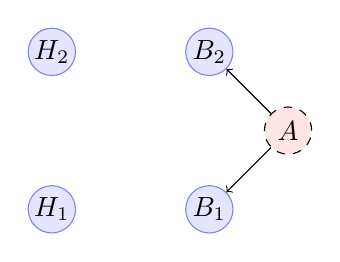
\begin{tikzpicture}
      \node[RV] at (-1,0) (H1) {$H_1$};
      \node[RV] at (-1,2) (H2) {$H_2$};
      \node[RV] at (1,0) (B1) {$B_1$};
      \node[RV] at (1,2) (B2) {$B_2$};
      \node[RV,hidden] at (2,1) (A) {$A$};
      \draw[->] (A) -- (B1);
      \draw[->] (A) -- (B2);
    \end{tikzpicture}
    \caption{The Bayesian network for the prediction problem for a fair coin. The probability of correct predictions depends only on $A$.}
    \label{fig:dbn-uncertain-Randi}
  \end{figure}

  2.
  \begin{align}
    P(B_1) &=  P(B_1 \mid A) P(A) + P(B_1 \mid \neg A) P(\neg A)  \approx 2^{-16} + 1/2\\
    P(B_2) &=  P(B_2 \mid A) P(A) + P(B_2 \mid \neg A) P(\neg A) \approx 2^{-16} + 1/2,
  \end{align}
  so $P(B_1) = P(B_2)$.
  
  3. We need to calculate the following function
  \begin{align}
    P(B_2 \mid B_1)
    &=  P(B_2 \mid A, B_1) P(A \mid B_1) + P(B_2 \mid \neg A, B_1) P(\neg A \mid B_1)\\
    &=  P(B_2 \mid A) P(A \mid B_1) + P(B_2 \mid \neg A) P(\neg A \mid B_1)
    \\
    &=  1 \times P(A \mid B_1) + \frac{1}{2} \times [1 - P( A \mid B_1)].
  \end{align}
  So we just need to evaluate:
  \[
  P(A \mid B_1) = \frac{P(B_1 \mid A) P(A)}{P(B_1)} = \frac{1 \times 2^{-16}}{ 2^{-16} + 1/2} = \frac{1}{1 + 2^{15}} \approx 2^{-15}
  \]
  We can now replace:
  \[
    P(B_2 \mid B_1)
    = 2^{-15} + \frac{1}{2} \times [1 - 2^{-15}]
    \approx \frac{1}{2} + 2^{-15},
  \]
  so a slight increase!
\end{proof}



\begin{exercise}
  We continue the previous exercise, but with the following extra assumption.
  \begin{assumption}
    Your utility for money is linear, i.e. $U(x) = x$ for
    any amount of money $x$.
  \end{assumption}     
  \begin{enumerate}  
  \item At the beginning of the experiment, JR bets you 100 CU that he can predict the \emph{next four} coin tosses, i.e. he is willing to give you 100 CU if he doesn't predict all four tosses. How much are you willing to bet against that, i.e. how much are you willing to pay if he does predict them correctly?
  \item You throw the coin 4 times, and JR guesses correctly all four
    times. Randi now bets you another 100 CU that he can predict the
    \emph{next} four coin tosses. Up to how much would you bet now?
  \end{enumerate}
\end{exercise}



\begin{proof}
  For this exercise, we simply need to calculate the expected utility. If JR can predict perfectly, then he has a chance of $1$ of predicting. If not, then he has a chance of $2^{-4}$. Marginalising over our prior:
  \begin{align*}
    P(B^4) &= P(B^4 | A) P(A) + P(B^4 | \neg A) P(\neg A)\\
             &=  1 \times 2^{-16} + 2^{-4} \times (1 - 2^{-16}) < 2^{-16} + 2^{-4} \leq 2^{-4} < 1/2
  \end{align*}
  Since our utility is linear, we should take the bet if $P(B^4) < P(\neg B^{4})$, which the above satisfies. We repeat the calculation for $P(B^{5:8} | B^4)$. Note that
  \[
    P(A | B^4) = P(A) P(B^4 | A) / P(B^4) \approx 2^{-16} /[2^{-16} + 2^{-4}] = 1 / [1 + 2^{12}] \approx 2^{-12}.
  \]
  Plugging in:
  \begin{align*}
    P(B^{5:8} | B^4) = P(B^{5:8} | A) P(A | B^4) + P(B^{5:8} | \neg A) P(\neg A | B^4) =  1 \times 2^{-12} + 2^{-4} \times (1 - 2^{-12}) \leq 2^{-12} + 2^{-4} \leq 2^{-4} \leq 1/2.
  \end{align*}
  So, we still should be more than sure that JR is not psychic even after 4 straight tosses and hence take the bet.

  \textbf{Note:} Of course, we are not being very careful here. We only considered the possibility that JR is a psychic or not. We haven't considered the possibility that JR may be performing a magic trick. This alternative hypothesis may have a much higher prior probability than JR being psychic.
  
\end{proof}

\begin{exercise}[DO NOT HAND IN]
  Now assume that JR is a psychic, but that he can only predict some proportion $\theta \in [0,1]$ of tosses (he could also be a \emph{bad} psychic).
We shall model our uncertainty about $\theta$ with a Beta distribution $\bel(\theta)$ with parameters $(2, 1)$, $\Beta(2,1)$, which places higher probability on all values of $\theta$ closer to $1$. So now our prior looks like this:
\begin{align}
  P(A) &= 1\\
  P(B \mid A) &= \int_0^1 P(B \mid \theta) \bel(\theta) d\theta = \int_0^1 \theta \bel(\theta) d\theta = \E_\bel \theta.\\
\end{align}
So now we know that JR is psychic, but not how good a psychic he is.
\begin{enumerate}
\item What is the resulting posterior distribution $P(B_2 \mid B_1)$ of JR predicting the next toss correctly after he has predicted one correctly? Write this in terms of the resulting Beta posterior parameters, given that $P(A) = 2^{-16}$.
\item Write an expression for the marginal probability $P(B_{n+1} \mid B^n)$, where $B^n$ is the event that he has predicted correctly $n$ times.
\end{enumerate}

\end{exercise}

\begin{proof}
  \begin{align*}
    P(B_{n+1} \mid B^n)
    &=  P(B_{n+1} \mid A, B^n) P(A \mid B^n) + P(B_{n+1} \mid \neg A, B^n) P(\neg A \mid B^n)\\
    P(B_{n+1} \mid A, B^n) &= \frac{2 + n}{3 + n}\\
    P(B_{n+1} \mid \neg A, B^n) &= \frac{1}{2}\\
    P(A \mid B^n)
    &=  \frac{P(B^n \mid A) P(A)}{P(B^n \mid A) P(A) + P(B^n \mid \neg A) P(\neg A)}\\
    &=  \frac{1 \times 2^{-16}}{1 \times 2^{-16} + 2^{-n}(1 - 2^{16})} \approx 2^{n-16}, \quad \textrm{for  $n <16$}\\
    P(B_{n+1} \mid B^n) &\approx \frac{2 + n}{3 + n} 2^{n - 16} + \frac{1}{2} (1 - 2^{n - 16}).
  \end{align*}
  So as we can see, the rate approaches that of the Beta model exponentially fast, even though the Beta model itself only has a polynomial rate approaching to one.
\end{proof}

\begin{exercise}
  The following is an example of a \emph{hierarchical model.}
  Instead of assuming that Randi is either a perfect psychic or a fraud, we can relax our assumption. Let $A$ denote the event that Randi is psychic, but that he can only predict some proportion $\theta \in [0,1]$ of tosses (he could also be a \emph{bad} psychic).
We shall model our uncertainty about $\theta$ with a Beta distribution $\bel(\theta)$ with parameters $(2, 1)$, $\Beta(2,1)$, which places higher probability on all values of $\theta$ closer to $1$. So now our prior marginal distribution looks like this:
\begin{align}
  P(B) &= P(B \mid A) P(A) + P(B \mid \neg A) P(\neg A)\\
  P(B \mid A) &= \int_0^1 P(B \mid \theta) \bel(\theta) d\theta = \int_0^1 \theta \bel(\theta) d\theta = \E_\bel \theta\\
  P(B \mid \neg A) &= \frac{1}{2}.
\end{align}
So now we think that JR is either a psychic or not, but if he is a psychic, we don't know how well he can predict. Still, we place a special emphasis on the case that he is not a psychic, where we'd expect him to predict correctly 50\% of the time.
\begin{enumerate}
\item What is the resulting posterior distribution $P(B_2 \mid B_1)$ of JR predicting the next toss correctly after he has predicted one correctly? Write this in terms of the resulting $P(A \mid B_1)$ and the resulting Beta posterior parameters, given that $P(A) = 2^{-16}$.
\item Write an expression for the marginal probability $P(B_{n+1} \mid B^n)$.
\item Randi now offers you the opportunity to bet 100CU at every time step $t$ that he would guess the next coin toss, with equal odds (i.e. you get 100CU if he doesn't guess correctly and lose 100CU if he does). If you accept the bet at time $t$, you throw the coin and Randi guesses, and you get/pay money depending on the outcome. Then he offers another bet at time $t+1$. If at any time you decline the bet, the game stops. Define a strategy for playing this game.
\end{enumerate}
\begin{proof}
  Here I offer a high-level sketch. The main idea is to calculate a posterior distribution on $A$ given the observations $B$. This can be written as follows:
  \[
    P(A \mid B)
    = \frac{P(B \mid A) P(A) }{P(B)}
  \]
  We can then replace the expressions for $P(B \mid A), P(B)$ and obtain the posterior distribution as usual. The rest of the exercise follows trivially.
\end{proof}

\end{exercise}








\fi

\end{document}

%%% Local Variables:
%%% mode: latex
%%% TeX-master: t
%%% End:
